\chapter{\label{chap:ethnoField} Joint action in context}

\minitoc




\begin{CJK}{UTF8}{gbsn}



\section{The Captain's speech at the first team banquet}

  The team dinner, organised at a restaurant adjacent to the Institute, was the first team ritual orchestrated by the new head coach Wang Chongyi. Following the abrupt departure of previous head coach Zhu, Wang thought it necessary to signal a new start for the team under his leadership as coach, and so he initiated a team banquet highly organised ceremony of eating, drinking, and speeches.

  I arrived late to the dinner after all athletes had already been seated, but the ceremonies had not yet started.  I noticed that many of the junior athletes appeared nervous and up-tight. More than 20 athletes were crowded around a single large (but not quite large enough) banquet table.

  Head coach wang sat in the position opposite the entrance to the private dining room (the equivalent of the ``head'' of the circular table).  Either side of Wang sat Han and Lu (the assistant coaches) and then the senior athletes in order of seniority, all the way until the opposite side of the table, where the most junior athletes were positioned.  Wang began the proceedings with three toasts (customary as the host), and then from there the senior athletes spoke in turn.  After each toast, the entire team had to drink a portion of their rice wine (and then beer after the rice wine had been drunk).  After the senior athletes had all had a chance to talk, the coaches directed each vague cohort of athletes (i.e., the very youngest athlete on trial, the aspiring Chaoyang students, the unruly undergraduates, and then the remaining senior team) to stand up and say a few sentences and then drink to the coaching staff (and senior athletes).

  The proceedings were relatively rigid to begin with, and from my position to the side of the table, the scene resembled an awkward face-off between the senior athletes and coaches at one end of the table, and junior athletes on the other end.  But once the effects of the alcohol kicked in, social interaction began to flourish. Speeches became bold and fluid with both self-assertive pronouncements and self-critical admissions, and the spaces between formal toasts were filled with one-on-one sideline conversations between athletes and coaches in which junior and senior athletes intermingled.

  Han Xiaolong's first speech, which came directly after Wang's three toasts, was one of the most bold and noteworthy for the purposes of highlighting the role of personal cultivation in group membershi
       \begin{quote}
         I don't know if all of you have your own personal goal?  I at least know that I have a goal, and that is to win next year's National Games gold medal.  That is what motivates me; that is what I am sacrificing for.  I don't know exactly what your goals are, but if you don't have a goal then your (personal) goal should be to help me achieve my goal.  I toast to everyone helping me achieve my dream [of winning a National Games gold medal]!
       \end{quote}
       \begin{quote}
           我不知道你们都有自己的目标吗? 我至少知道我有一个目标,那就是拿到明年全运会的金牌。 这就是我的动力,就是我所牺牲的。 我不确定你的目标是什么,但如果你没有目标,那你的目标应该是帮助我实现我的目标。 我向所有人致敬,帮助我实现自己的梦想!
       \end{quote}

  I was automatically struck by these remarks speech. I suspect that the intuitions around team membership that I had generated in rugby contexts elsewhere prepared me for a speech in which Han would seek to embody an egalitarian notion of group membership. Han was the most senior athlete in the team, he was the former team captain and was now in transition to coach.  ``We are all equal under the category of the team,'' he ought to say; we are all in this together (aren't we)?  Instead, in his prime-time team captain talk, Han was intuitively compelled to demonstrate the strength of his own personal conviction as a means to in order to foster team solidarity.




\section{Introduction}

In this chapter, I present ethnographic evidence that serves to situate a general account of team click in group exercise in the context of professional rugby in China.  In particular, I explain the way in which athletes of the Beijing men's rugby team experience uncertainty in joint action, and the extent to which uncertainty can be associated with physical and social coordination.

Ethnographic evidence suggests that athletes' general unfamiliarity with rugby prior to arriving at the Institute, and high variation in athlete technical competence within the team, will mean that rugby's joint action may be experienced as challenging, owing to its high levels of uncertainty.  Based on the prediction that more successful team performance in joint action will require more coordination of physical movement and social communication when uncertainty is higher \citep{Riley2011}, it can be expected that athlete experience of on-field physical coordination and off-field social interdependence will be salient and meaningful to athlete experience.

In this chapter I demonstrate that, despite strong utilitarian motivations for adherence to rugby, such as access to coveted life-course opportunities such as education and employment, athletes nonetheless experience enjoyment, interdependence, and group membership associated with rugby's joint action.  Where relevant, I draw attention to the the role of a Chinese relational mode of cognition in shaping these observable processes.  In sum, by describing the contours of uncertainty and coordination in joint action, I am able to render a general account of team click in group exercise testable (Chapter~\ref{chap:ethnoResults}).





\section{Experience of uncertainty in joint action\label{sect:uncertaintyJA}}

A range of ethnographic evidence suggested that uncertainty was salient to athletes' experience of rugby's joint action.  It soon became obvious that rugby's joint action requirements posed a significant challenge for athletes attempting to learn the game from scratch.  During semi-interviews, within the general theme questioning regarding of the costs and benefits of adherence to rugby, I asked athletes what they thought was ``the most difficult part of rugby'' (你觉得橄榄球最难的一部分是什么).  I deliberately left the question open to interpretation, and if asked to clarify, I followed up by using the compound \textit{kunan} (困难), to emphasise the challenging dimension of difficulty, i.e. ``what is the most \textit{challenging} part of rugby?'' (橄榄球最\textbf{困难}的一部分是什么?).  In his interview, senior athlete and Beijing local Su Hailiang summed up the feeling of being a new athlete without any foundation in rugby:

      \begin{quote}
          I think the hardest thing---well it was all really hard.  At the time when I couldn't do anything, when my body development wasn't that good, I wasn't that strong.  Basic skills, ball skills, planned moves, etc. [were all not very good].
      \end{quote}
      \begin{quote}
          我觉得最困难的,都挺困难的,当时什么都不会,身体素质也没那么好,没有那么强壮,也没有那么好,身体素质。基本功、球技、记战术什么的。
      \end{quote}

This passage suggests that an athlete's initial induction into the rugby program could be overwhelming due to rugby's many diverse requirements.  As unruly undergrad Fang Chao explains:
                \begin{quote}
                The hardest thing about rugby is all of the small details. Rugby is such a comprehensive sport, and playing in a real game is very different from training. I remember when was playing a tournament in 2014, at the time I had only just started training (for rugby).  As soon as I took the field my whole brain was blank.  Now I am a bit better, my vision is broader.
                \end{quote}

                \begin{quote}
                橄榄球最难的一部分是很多小细节吧。橄榄球是很全面的项目,打比赛跟训练还是有区别的。 14年的时候打比赛,那时候刚练,一上场整个脑子就空白了,现在会好一点,视野也开阔了。
                \end{quote}
In his response, Fangchao draws attention to the difficulty associated with the ``on-line'' and ``in-the-moment'' demands of joint action in rugby.  When he first started playing in real rugby matches, the pressure of being on the field and in the moment meant that there was no time for him to think or see.

Of the 20 athletes who responded directly to this question (in the remaining six interviews either I did not ask this question, or athletes did not respond to the question), all 20 interpreted it as a question about rugby's on-field demands.  12 athletes cited an aspect of rugby that related to on-field coordination of behaviour that pertained more to coordination with teammates:
Six athletes mentioned  ``awareness'' (\textit{yishi} 意识), three talked about on-field coordination with others (\textit{peihe} 配合), two talked about on field decision-making (\textit{panduan nengli} 判断能力), and two talked about planned running lines (\textit{paowei} 跑位) and team moves (\textit{zhanshu} 战术).
One mentioned pressure from the coach (\textit{jiaolian} 教练).
Six athletes cited an aspects that focussed more predominantly on individual-level  components of performance
Four athletes mentioned tackling (\textit{pulou} 扑搂) or individual defence \textit{geren fangshou} 个人防守) , two mentioned individual running speed (\textit{sudu} 速度), and two mentioned footwork in attack (\textit{jiaobu} 脚步).  One athlete reported fear of injury as the most difficult aspect about rugby.  The remaining two athletes cited both an aspect that was related to coordination of behaviours with others, as well as an aspect of individual performance.  These results suggested that athletes experienced a range of specific components as technically challenging, with a tendency to experience of on-line coordination with others, or team performance, as the most challenging aspect of rugby.

Here, I employ the terms team performance and individual performance to distinguish to modes of a spectrum of joint action in rugby (see ~\ref{sect:jointActionRugby}).
Team performance usually entails joint action that requires explicit coordination with teammates (such as coordination of attack and defensive line, passing between two or more players, etc).  Components of individual performance, by contrast, entails a focus on individual actions that contribute to larger joint action goals (such as tackling, individual passing, effectiveness in contact encounters at the breakdown, etc.)

%(outlined in Chapter~\ref{})
The detail of athletes' interview responses to the question of rugby's most difficult aspect suggested that  that team performance may be experienced as more challenging than individual performance.
  As Wang Zhenfeng, a tall and extremely talented (but still relatively inexperienced) senior athlete, explained:
            \begin{quote}
            For me, it's probably the decision making with ball in hand: after you get the ball, how do you create opportunities for others---I think that's especially difficult.  For me, I think breaking the line or attack or whatever...breaking the line or stepping and so on...I'm ok at all of these things [individual components of performance], but if you ask me to create an opportunity for someone else after I have broken the line---that's when I find it difficult.
            \end{quote}
            \begin{quote}
            对我来讲应该是球的分化,拿到球之后分化给别人创造机会我觉得特别难。我觉得突破或进攻还是干嘛的,去突变向什么的对我来说都还好,但是让我即能突然后给别人创造机会我觉得很难。
            \end{quote}
Here, it is not only the on-line and in-the-moment dimensions of rugby that Wang finds challenging, but also the fact that he must create opportunities for others.

Wang Zhankun, a young and promising kid student from Chaoyang school expressed a similar sentiment:
          \begin{quote}
          I'd say the ability to adjust to being on the field in a game.  When I'm on the field I can only see those few people who are close to me, when I'm tired I feel like I can't see anything, like there could be a gap, or an opportunity, but often I can see it.
          \end{quote}
          \begin{quote}
          场上的适应能力吧。我在场上只能看到离自己近的几个人,累的时候感觉看不到所有,可能空档啊、机会啊经常看不到.
          \end{quote}
These results suggested that on-field coordination of behaviour with others may have on balance been experienced as more challenging than action that required less dynamical coordination with others, such as passing or kicking the ball.

\myparagraph{On-field awareness}
Perceived challenge in rugby associated with developing on-field ``awareness'' (\textit{yishi} 意识) was a prominent response from athletes.  Of the 14 athletes who cited coordination of behaviour with others as the (or one of the) most difficult aspects of rugby,  six athletes mentioned awareness directly.  Of these six, five mentioned awareness (\textit{yishi}) and one specified ``continuous on-field awareness'' (在场上连续意识).  Awareness appears to describe an ability to cope with the on-line decision making demands of joint action in rugby.

Bao Yuhan, an unruly undergrad and Beijing local, expressed to his experience of the challenge of awareness on the field:
    \begin{quote}
    (I think its about) maintaining continuous on-field awareness.  Often I'm never thinking that many steps ahead.  Sometimes when I break the line, once I break through I can't keep on going.  Suppose like that one time in Shanghai in 2014, I gave the ball to Wang Zhenfeng and he broke through, and then no one followed him.  I stood there looking at him run from where I passed the ball, I was so tired I couldn't do anything... As soon as I realised what was happening, I was like ``Oh! Quick get after him!'' In the end we were one step away---only one step away from losing the ball.
    \end{quote}

    \begin{quote}
    在场上连续意识. 我总是想的不是那么多翻。有时候突破的时候,突破了不会再打。假如在上海14年我给王贞丰突破了,然后没人追上了,我在原地累得不行了看着,我一看,''哦!快追上!''最后差一步,就差一点会丢球。
    \end{quote}

Like Wang Zhankun above, Bao Yuhan also suggests that physiological fatigue has an impact on ability to maintain awareness.  Thus, in addition to the time pressure and cognitive complexity of joint action in rugby, the role of exertion and fatigue also appears to be relevant to an ability to think, see, and act clearly on the field.

An emphasis on on-line and in the moment team performance more so than components of individual performance over which an individual would have more control (e.g., passing or kicking the rugby ball), can be taken as evidence that athletes experience higher levels of uncertainty in rugby's joint as more difficult or challenging.

These passages taken from semi-structured interviews suggest that rugby's on-field demands in joint action place severe constraints on athletes' ability to be (consciously) aware of the environment around them, including the actions and intensions of others.

\myparagraph{Variation in technical competence}
Achieving awareness in rugby appears to be inherently difficult.  But athletes also suggested that it was something that could improve over time.  Senior player Cui Shuocheng, who had recently transferred from Shandong province team to Beijing, compared his relative lack of awareness to foreigners like me who had played the game from a young ag
      \begin{quote}
      Right at the start, when I was coming into the team, I couldn't play. I'd often watch the older players playing touch and thought they were so impressive.  At the time when I couldn't play at all, I thought everything was such a challenge  when to straighten up my passing line (in attack), when to pass the ball.  I would always lose awareness or just always stop. I couldn't compare with you foreigners, you have this awareness from a young age.  We have no solid foundation, we all transfer over from individual sports, and so I don't think we get it.
      \end{quote}

      \begin{quote}
      刚开始进队的时候不会打,经常打TOUCH看他们玩,觉得特别帅。当时我不会,当时就觉得特别困难,什么时候插上,什么时候穿球,意识方面老断老断,老停,跟你们老外没法比,你们从小就有这个意识,而我们半路出家,由个人项目到团体项目,觉得不了解.
      \end{quote}
In his description, Cui Shuocheng suggests that awareness relates to knowing both what action is required at what time.  Shuocheng insinuates that such awareness develops over time---preferably from a young age---so that awareness has a chance to become more automatic and immediate.

This line of reasoning raises the possibility that that athlete experiences of challenge and difficulty in joint action may have been associated with varying levels of familiarity with rugby's technical requirements.  First, in contrast to professional rugby players of traditional rugby playing nations, who grow up playing rugby from a young age (and thus accumulate technical competence and experience through years of playing and training), the members of the Beijing rugby team were all relatively new to rugby and to team sport more generally.   Due to Rugby's minnow status in China, most athletes started from scratch when they first arrived at the Institute—-some (like Hongwei) had not seen a rugby ball before they arrived.

Table ~\ref{tab:athleteDescriptives} describes athlete attributes such as average age, rugby training age, years spent in the team, and previous sport.  The average rugby training age (years spent playing and training in a rugby program, measured at time of semi-structured interview) was 3.34 years ($median = 3, range = 0.16 –-- 8 years, SD = 2.02$).

The distribution of training age reveals that over half of the sample had a training age of three years or less (see Figure ~\ref{fig:ethnoTrainingAgeHist}).
      \begin{figure}[htbp]
       \begin{center}
       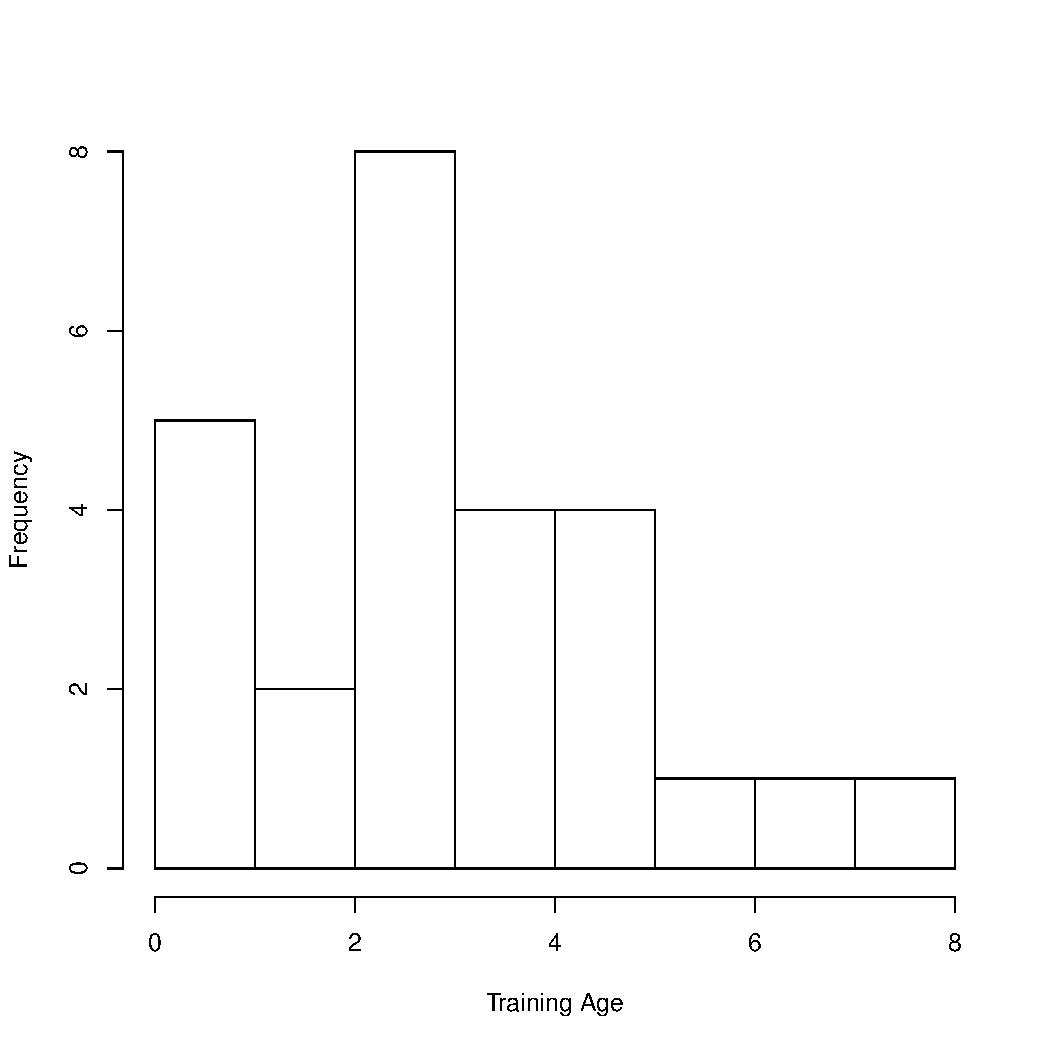
\includegraphics[scale=.3]{images/ethnoTrainingAgeHist.pdf}
         \caption{Distribution of athlete training age ($n = 26$)}
       \end{center}
         \label{fig:ethnoTrainingAgeHist}
      \end{figure}
18 of the 26 athletes had a background in other sports (16 athletes from track and field, one from football, one from basketball).

These athletes usually began part-time or full-time physical training at the age of 11 to 13.  Those who transferred to rugby from other sports did so either at the beginning of senior high school (16 years) or at university age (18 years).  The remaining eight athletes had no particular sporting background before rugby, and most began adherence to rugby at high school or university age (16---19 years).These athletes were either scouted by the head coach of the rugby Program or by school athletics coaches based on their basic athletic attributes (running speed, strength, coordination, and potential for physical growth).\footnote{Of the 26 athletes in the squad, three junior athletes who were part of the squad when I arrived in September 2015 left before August 2016; and three new athletes arrived during the time I performed research.  This flux of athletes in and out of the team was quite common, due to the fact that recruitment often occurred informally via personal networks}.  These data suggest that most athletes had been training for only a short time (relative to other professional rugby players of traditional rugby playing environments), and came a baseline familiarity with rugby (and team sports more generally) of vritually zero.  It is possible that this relative unfamiliarity with rugby's technical requirements can contribute to an explanation of athletes' experience of challenge relating to rugby's joint action.

In addition, the Beijing men's team also showed considerable levels of within-group variation in measures that could indicate technical competence or familiarity with rugby's joint action.  The team consisted of 13 athletes who were considered ``senior athletes'' (\textit{lao duiyaun} 老队员; training age = 4.57 SD = 1.65).  Of these 13 athletes, eight athletes were considered part of the most senior ``starting team'' (\textit{zhudui} 主队), the remaining five were considered part of the ``reserves'' (\textit{tibu} 替补).  Athletes were engaged by the Institute on varying levels of contract: one was a permanent employee (\textit{zhengshi} 正式)\footnote{Senior athlete Su Hailiang was the only permanent employee, by virtue of the fact that he was a Beijing resident.} and seven were full time contracted athletes (\textit{xieyi} 协议).  The remaining five senior athletes were provisionally contracted on a ``training contract'' (\textit{shixun} 试训).

The remaining 13 athletes were considered ``junior athletes''(\textit{nianqing duiyuan} 年轻队员; training age = 1.91 SD = 1.30)
Six junior athletes were engaged by the Institute on ``student level'' contracts (\textit{erjiban} 二级班), and the remaining seven trained with the program on a ``trial'' basis (\textit{jixun} 集训); effectively on a trial arrangement until they showed promise or else withdrew from the squad).  Athletes contracted as students did not receive a salary but received in-kind support in the form of training, food, board, and health insurance at the Institute.\footnote{Most athletes were from urban and rural areas of northern China (Shandong (11), Beijing (6), Jiangsu (3), Liaoning (2), Hebei (2), Henan (1), Heilongjiang (1))}.

The Beijing men's team contained distinct stratification according to training age and seniority, and it was possible that variation in training age and seniority was associated with experiences of uncertainty in joint action.  I discuss this possibility in more depth in the following chapter.  Here, it is important to note that the sample of athletes with whom I conducted research contained high within-group variation in measures that denote technical competence.  This natural variation was useful for the purposes of comparing and contrasting athlete experience of joint action.


In sum, these data confirm the proposal that rugby poses a serious challenge to the goal of successful joint action.  Unprompted, athletes drew attention to the in-the-moment and time-pressured nature of joint action in rugby.  It appears as though, on the field at least, there is no room for thinking.  According to athlete testimonies, there appears to be very little room for ``seeing,'' too.  Vision is reduced to the immediate surrounds, and this reduction in awareness constrains the extent to which athletes can identify optimal action selection in multi-agent interaction.  Athletes were on average more fixated on the difficulties associated with coordinating with others.  Individual level components of performance such as tackling and side stepping were also prominent concerns—and these components shared with team performance an on-line, in-the-moment quality.   In addition, athletes suggest that physiological fatigue can also play a role in reducing awareness.  From these results I infer that perceptions of on-field team performance as more difficult than other forms of action is an indication that athletes' experience uncertainty in rugby's joint action, defined as an inability to predict, establish, and sustain joint action.







\section{Coordination}
The results presented above suggest that athletes experience rugby's joint action inherently challenging.  Team performance appears to be more challenging than individual performance, and successful team performance required ``awareness'' — a tacit and immediate sense of knowing what to do on the field without having to think about it.  I infer from this evidence that uncertainty of joint action in rugby is salient to athletes.

As stated above, the general theoretical account of team click in group exercise is predicated on a dynamical link between uncertainty coordination.  In other words, uncertainty in joint action will demand coordination—--of physical movement and social communication---in order for joint action to occur successfully.  In this section, I consider ethnographic data that could evidence for this link, in order to set the foundation for an assessment of research hypotheses in the next chapter.

As I explain below, deciphering evidence for coordination—--of both on-field physical movement and off-field social communication—--proved to be an intricate challenge owing to what appeared on the face of things to be competing athlete motivations for adherence to rugby.   In essence, evidence suggested that attention to fostering on-field and off-field (social) coordination was secondary to more immediate concerns relating to strategic life-course opportunities and cultivating social networks external to the team.  However, a triangulation of ethnographic data and theory derived from a Chinese relational mode of social cognition helps decipher more nuance in this picture.

I suggest that that motivation for coordination existed in spite of (and/or alongside) competing motivations for the strategic pursuit of life-course opportunities of eduction and future employment.  Rather than being understood as competing, these motivations can be understood as deriving from affordances that intersect in this particular setting.  While almost all athletes arrived at the Institute with the explicitly-defined motivation of ``family and education first; team second,'' many left the institute with a deep, visceral and socially agentic connection to rugby, their team mates, and coaches.


\subsection{Evidence to suggest that strategy and \textit{guanxi} compromised team coordination}

Various strands of ethnographic evidence suggests that, on the face of things, athlete adherence to rugby was motivated primarily by the pursuit of strategic life-course opportunities of tertiary education and future employment.  Evidence from a survey performed after each semi-structured interview revealed that athletes declared their family and pursuit of education as the primary motivations for adherence to rugby.

Upon completion of each semi-structured interview, I asked athletes to complete an activity in which they were asked to rank (from most important to least important) their motivations for adherence to rugby at the Institute.  I selected these motivations based on preliminary unstructured interviews and conversations with athletes, coaches, and other knowledgeable observers.  The motivations included: ``Education'', ``For Beijing'', ``Family'', ``Gain Respect of Others'', ``For Teammates'', ``Employment'', ``Beijing Residency'', ``Money'', ``Enjoyment'', ``Popularity (with prospective romantic partner).'' I wrote each motivation down on a piece of paper and scattered them randomly on the surface of a table in my room where I conducted interviews.

Mean rank of motivations for adherence to rugby revealed a clear trend that family and education were the most prominent motivations for adherence to rugby (see ~\ref{tab:athleteMotivations}).  When asked in semi-structured interviews, almost all athletes agreed that their most prominent explicit motivation for playing rugby was to pursue life-course opportunities of education and employment.  Importantly, it was also commonly declared that achieving education and employment through commitment to rugby would make their families proud.  In addition, ``to gain respect from others'' also featured as a prominent motivation—a result that echoed athlete testimonies that rugby was a revered and respected pursuit in their social circles beyond the institute.  In this instance it was difficult to claim that rugby itself was the source of respect from others.  Indeed, given the prominence of education as a motivating factor, reverence for rugby may be tied up in the fact that adhering to rugby at the Institute signals close proximity to the achievement of attending a prestigious university such as BSU.

Very few athletes ranked ``enjoyment'' as a primary motivation.   It would not be inconceivable to see this as a strongly cited motivation for adherence to rugby in settings in which rugby exists as a popular mainstream sport.  Many, including some professional practitioners would claim to be adhering to a sport like rugby simply ``for the love of the game'' \citep{Jackson1998}.  Money, Beijing residency, and attracting a romantic partner associated with adherence to rugby were all less relevant to athlete concerns.  When forced to rank motivations for adherence to rugby, life-course opportunities and family were on average more dominant than motivations driven by team-based categories such as ``For Beijing'' (4th) or ``For Teammates'' (6th).
                    %\begin{table}
                     % Please add the following required packages to your document preamble:
% \usepackage{booktabs}
\begin{table}[]
\centering
\begin{tabular}{@{}clc@{}}
\toprule
\textbf{Rank} & \multicolumn{1}{c}{\textbf{Motivation}} & \textbf{Mean (SD)} \\ \midrule
1             & Family                                  & 2.34 (2.35)        \\
	          &          	                            &        \\
2             & Education                               & 2.38 (2.19)        \\
	          &          	                            &        \\
3             & Respect                                 & 3.50 (2.61)        \\
	          &          	                            &        \\
4             & Represent Beijing                       & 3.58 (2.04)        \\
	          &          	                            &        \\
5             & Employment                              & 3.96 (2.04)        \\
	          &          	                            &        \\
6             & Teammates                               & 4.00 (1.94)        \\
	          &          	                            &        \\
7             & Enjoyment                               & 5.69 (3.16)        \\
	          &          	                            &        \\
8             & Money                                   & 5.85 (2.22)        \\
	          &          	                            &        \\
9             & Beijing residency                       & 6.42 (2.61)        \\
	          &          	                            &        \\
10            & Attract a partner                       & 8.00 (1.41)        \\ \bottomrule
\end{tabular}
\caption{Athlete motivations recorded following semi-structured interviews (n = 26)}
\label{tab:athleteMotivations}
\end{table}

                     %\end{table}

Senior athlete Lu Peng explained to me the prominence of education as a motivation for adherence to rugby:
      \begin{quote}
          Yeah, most of us in Shandong are like me, 80-90\% are of the same idea: there is an awareness that individual sports need less people, and so coming to rugby this type of team sport, most people's goal is to use rugby to get to university.  But when I came to CAU I thought suddenly that I really like this sport, before I had never come into contact with a team sport before, and it was a team sport involving a ball, so I really liked it.
      \end{quote}
      \begin{quote}
           对,因为我们山东大部分人,都是像我这种,百分之八十到九十差不多都是这个思想,就是这么个意识就是说,单项需要人少,所以来橄榄球这类集体项目,大部分目的就是为了上个学。但是来到了农大之后我觉得我突然就喜欢这个项目,以前没接触过集体项目,而且有球的集体项目,所以我很喜欢。
      \end{quote}
At the same time as citing the more obvious strategic motivation for adhering to rugby, Lu also admits that he immediately came to like and enjoy rugby once he began to train at CAU. I will discuss this feature Lu's testimony—also common to many others'---in more detail below.  Here the main point is that the overriding motivation that lands athletes in rugby programs all over China is `` family and education'' first.
These results suggested that athletes who were motivated more by strategic life-course opportunities and familial social networks beyond the team, may have been less less motivated to attend to team concerns, for example, of on-field coordination of physical movement and off-field social communication.

\myparagraph{Impact of strategic motivations on impact and mood}
In addition to survey data and athlete testimonies in interviews, I also observed a number of instances in which an athlete's mood fluctuated according to the state of their attempts to secure life-course opportunities of education and employment.  Often the path to securing entrance to BSU was not always straightforward, even if athletes had earned the ``Master Sportsperson'' prerequisite.

Two senior athletes, Ma Haitao and Cui Suocheng, despite both long qualifying as Master Sportspersons, were involved in complex bureaucratic journeys in an attempt to gain admission to BSU.  One day early in my first stretch of ethnography, I was taking a training session in which we were focussing on defence, and Shuocheng suddenly appeared to have given up all energy.  All of a sudden stopped doing the prescribed tackling drill.  I took him aside and began to take him through some of the details he missed last week when he was away.  He refused to listen and said, ``I get it, I just don't want to do it, I'm sick of it, I've had enough of this drill'' (我知道怎么练,我就不想练了。练够了!)''You've had enough?'' I asked, ``Alright, if you've had enough then get off the field!'' (练够了?好吧,那你靠边去!).  I snapped at him, motioning to the stands for him to go and sit down. I was stunned that he said that he didn't want to practice; I was even more surprised when Shuocheng immediately followed my instruction and sat on a tackle bag on the side of the training field.  Later on in the training session, he came back over to the subsequent training drill and started offering (helpful) advice to the more junior athletes about their technique.

A few days later I found an opportunity on our way back from training to the dormitory to ask head coach Zhu about the situation with Shuocheng.  Zhu explained that Shuocheng was experiencing difficulty finalising his contract transfer from Shandong to Beijing province, and that this procedure was interrupting his ability to process his university application (Shuocheng had moved from Shandong provincial team in 2014). To attain prized life-course opportunities through adherence to rugby was obviously a core motivation for most athletes. At times for some, the issue became critical enough to seriously these impact on athletes' on-field performance.

Ma Haitao, another senior athlete also in the process of trying to apply for university (after years of delays), also experienced large amounts of stress during my time researching.  One day he spoke to me at length about the way in which these difficulties were impacting on his mood and his ability to focus on training. ``It impacts me so strongly'' (对我的影响太厉害了) he said as we walked to the canteen after a training session. ``I'll probably need to have a long sleep or take a break from training before I can recover from these sort of frustrations---the endless process of getting this form and completing that form, its so frustrating.'' (我可能要先睡个好觉请假休息才能回复过来呢。这个那个证,跑断腿盖章了,令人太沮丧了.)  These examples were representative of many more instances in which it was clear that athletes attended prominently to the education as the primary motivation for adherence to rugby.  The goal of gaining entrance to BSU appeared to bear directly upon athlete ability to contribute to the activities of the team, including on-field coordination of movement.

\myparagraph{Strategic motivations were used to explain poor on-field performance}
Strategic motivations were also often used by more senior athletes or coaches to explain poor on-field performance.  An example of this pattern occurred a few weeks into my first stretch of research.

After a few weeks of observing training and a few sessions in which I myself took the team for training, the different factions in the team became quite clearly expressed on the field.  Generally speaking, the trialists were either on the sidelines learning and practicing the basics, or very tentatively beginning to join regular team drills in which all other athletes participated.  From my position of expertise it was clear to see that, of those athletes who trained regularly, the old-guard of Han Xiaolong and Lu Peng were the most experienced athletes.  Below them, the rest of the senior athletes varied in competence according to experience and individual differences, and student athletes from Chaoyang School were noticeably less experienced than their more senior counterparts.

The structure of training drills reflected constraints due to high within-group variation in technical competence.  Training drills were usually structured in such a way that athletes of similar abilities almost always trained together in the same subunits, rather than randomly assorting into subunits for each training drill (as was normal practice in rugby training sessions I had become accustomed to outside of China).  This tendency to group according to seniority and competence was most obvious in a basic passing drill involving four athletes per subunit (in which athletes would pass the ball between each other while running up and down the field.  Usually the most senior four athletes present at that training would naturally form the first subunit, followed by the next most senior (or competent), and so on, until the most junior and least competent or experienced athletes would form a subunit and attempt to emulate the preceding subunits.

When talking to senior players about this custom in training, I was told that the habit was necessary for two factors.  First, given that the differential in ability between the most senior and most junior athlete was so large, sorting according to seniority and competence (as opposed to randomly) ensured that the senior athletes could achieve a basic level of quality in their practice.  Second, by sorting together in sub units and doing the drill first, senior athletes could demonstrate the ideal standard for execution of each drill for the rest of the team to emulate.  Thus, on-field coordination in joint action appeared to be fundamentally constrained by within-group variation in athlete technical competence.

Interestingly, I began to notice variation in team performance at training according to which athletes (or coaches) were present.  After a few weeks of observing training I eventually began to coach the team myself, focussing on defence and ``contact'' work, and team play.\footnote{Contact refers to skills of rugby that involve body-on-body physical contact in addition to defence.}  For the first few weeks, athletes showed obvious dedication and conscientiousness when participating in training and learning the new content that I taught them.

One day approximately two weeks after I first started coaching the team,  I took a session in which for the first time almost all the senior athletes were unable to train, either due to injury or other commitments such as attending BSU for university matters.  The impact on the quality of training was palpable.  The junior athletes who were present were, for whatever reason, passive and unresponsive to instructions, and appeared unable to provide direction to the athletes below them.

Over the course of my research, a clear pattern emerged, in which the quality of training was more or less correlated with participation of senior athletes. Without senior athletes helping direct training, athletes---particularly the more junior athletes---were generally slower to react to new information.  One day a few weeks after noticing this pattern, I took an opportunity to consult the assistant assistant coach Shi and senior athlete Han Xiaolong about the issue.  Coach Shi proposed his opinion on the situation:
      \begin{quote}
     Some athletes think its ok to just be an athlete here and get to BSU, and not pursue anything higher or anything more.  Actually, it's ok to think like that. But if that's the case then sorry, you'll have to watch from the sidelines.
         \end{quote}
        \begin{quote}
             有的球员觉得好在这当运动员上体大就可以了,不去追求更高的更多的。其实,可以这样想,但是,对不起,你要靠边看着。
         \end{quote}
When talking to the senior athletes and coaches about the quality of training (or lack thereof), the most problematised of all the team factions was the group of ``training contract'' athletes, most of whom had just begun their undergraduate studies at BSU.  The basic consensus was that these undergrads lacked initiative and focus; they were too distracted by university, computer games, and pursuing romantic love. Having achieved the core goal of gaining access to university, the ``unruly undergrads'' were often criticised for not possessing sufficient intrinsic motivation to dedicate them to rugby.

Lu Zhongsheng (or ``Big Mouth Monkey'' (大嘴猴) as he was affectionately for his gregarious and cheeky personality and his big mouth) produced a similar critique of the team's more junior athletes:

      \begin{quote}
        [The problem with the junior athletes is that they are] immature, always thinking that they should be training for us rather than training for themselves.  They think: ``here I can take a monthly salary of a few thousand RMB''---they think that just ``getting by'' is fine.  They think, for exampl  ``I have already got in to university, as long as I graduate then I don't really mind, after all I've already made it to university.''  This is immature.  Wait until the day you become like me and you've got nowhere else to go, then you'll...since you've already chosen this sport, then you'll finally want to work hard at it, to train hard, to achieve some sort of goal.  Its like you said [referring to the researcher], they think that if the coach is watching me, then I should train hard; if the coach is not watching me,then I won't train hard...\\

        Before when I was living with Elder brother Han (Han Xiaolong) in the same dorm room, every night after we would have to hand in our mobile phones, we would talk for ages about these rugby questions. But other teammates maybe aren't like that, they will probably talk about computer games, girlfriends, or bloody random and unimportant things.  They're always talking about this... If you wanted them to talk about rugby then maybe they'd... I don't understand it anyway.
      \end{quote}

      \begin{quote}
        心态不成熟,总觉得是为你训练而不是为自己训练,我在这每月拿几千块钱的工资,感觉混一天是一天。比如我已经上学了,只要大学毕业了就无所谓了,反正我已经上学了。还是不够成熟,等到有一天像我一样无路可退的时候就会。。。你既然已经想选择这个项目,你要去努力, 好好训练,要做出一种成就。如果像你说的那样,教练看着我就好好练,教练不看我我就不好好训练...我
    以前跟龙哥一屋,每天晚上不是要交手机么,然后我们两个人会谈论很久这些橄榄球的问题。但是别的队员可能不会这样,他们可能就会谈一些游戏啊,女朋友啊,乱七八糟的琐事和小事。他们每天都谈到这个。你要是让他们谈到球可能。。。反正我很不理解。
      \end{quote}

Lu's rant about the unruly undergrads was representative of many instances in which I observed more senior athletes explain an athlete's lack of contribution to team performance in terms of a lack of motivation. Here, it is inferred by Lu that the undergraduates lack motivation to contribute to team performance because they are more fixated on the primary motivation of attending and, it would seem, enjoying university (computer games, girlfriends, etc).

I return to the nuances associated with rationales for poor team performance in the following chapter (see Chapter ~\ref{chap:ethnoResults}).  For now, suffice to say athletes and coaches alike suggested a relationship between motivation for strategic goals such as attaining education and poor team performance.   In effect, these motivations were assumed to conflict with and detract from the motivation for successful team performance, i.e., on-field coordination.


\myparagraph{The team as a platform for strategic interests}
I noticed a number of instances in which it appeared that the team was used as a platform for strategic interests that ultimately detracted from on-field coordination.

The relatively sudden change in head coach half way through my first stretch of ethnographic research gave me the fortunate opportunity to witness the implications of this transition for the social organisation of the team.  When I returned to Beijing after a 10 day travel break in February, almost a month after head coach Wang had replaced former head coach Zhu, two of the athletes who were on trial under Zhu's tenure---Xu Gong and Lian Jianxiang---had since left.  When I asked senior athlete Wang Wei about the disappearance of these two students, he suggested that ``they had interests with Old Zhu...Old Zhu said that he could solve their ``school problems'' [i.e. get them into university]. They were here to try to get in to University.'' (和老朱有利益关系,老朱说可以解决上学的问题 都是过来上学的).
Talk of ``grey'' arrangements of this nature in sport in China was hushed but common, but it still came as a shock to me.

Taken together, this evidence suggests that the link between uncertainty and coordination as a response to uncertainty may have been dampened or challenged at times by competing or overriding motivations to pursue strategic life-course opportunities of education, or to attend to more dominant concerns associated with fostering a hierarchical network of relationships (\textit{guanxi}).


\subsection{Coordination existed in relational terms}
Evidence reviewed in the section above suggests that, in the case of the Institute, the foundational theoretical claim that underwrites a general account of team click in group exercise may have been threatened.  The possible link between uncertainty and coordination in joint action appeared to be at times disrupted by the existence of strategic activities and extra-team priorities.  Do these findings suggest that, in which case, team click was not likely to be found among athletes at the Beijing men 's rugby team? Or, was it possible that in real world scenarios such as this one, the relationship between uncertainty and coordination was much more nuanced multi-faceted?

In this section, I review evidence to suggest that concerns for team coordination existed, and indeed were powerful sources of motivation in spite of (or indeed, alongside) strategic motivations of athletes, coaches, or officials.  With assistance from theory deriving from a relational mode of social cognition \citep{Liu2009}, it is possible to see that concerns for team coordination existed in forms that were more relational than categorical.  Re-examined with a relational lens, many prima-facie strategic or utilitarian behaviours referred to above can also be understood to contain dimensions of concern for social coordination.  As I will explain below in reference to on-field team performance and off-field processes of group membership, the uncertainty of joint action may have been addressed by Beijing athletes ways that were less immediately obvious to me as a researcher.


\subsubsection{Responsibility for team performance is distributed throughout an hierarchical network of relationships}
To return to the example poor training performance in the absence of more senior players. I found evidence to suggest that Coach Shi's rationale for junior athletes' lack of motivation may have been insufficient.  In particular it did not take into account the hierarchical and relational structure of on- and off-field activities to which athletes at the Institute were subject.

Immediately following Coach Shi's rationale for poor commitment at training, Senior athlete Han Xiaolong offered a different interpretation, by suggesting that the undergrads were becoming habitually un-focussed during training:
     \begin{quote}
       It has become a habit.  When we were at CAU, at that time during university, we would also lack focus at times and so on, but back then, as soon as head coach Zheng would take training, we would all be immediately focussed!
      \end{quote}
      \begin{quote}
       成为一种惯性,我们在农大那个时候也会不关注等等,但是那个时候郑老师一带我们就全在关注
      \end{quote}
Coach Zheng was---at the time that Han was referring to---the most authoritative coach in Chinese rugby (see Chapter~\ref{sect:rugbyInChina}). The tales of Zheng's intensity as a coach were infamous (see Lu Peng's description of video analysis in Chapter~\ref{sect:openScrutiny}), and it was clear based on older athletes' recollections that Zheng's presence alone was enough to inccite deep anxiety-induced focus from athletes.

Senior athlete Lu Peng, who had also been coached by Zheng Hongjun, tained an exchange that powerfully summarises the agency of the coach in directing behaviour in joint action.  At one point in the interview, we arrived at the conversation of the role of the coach in the team, particularly the idea that if athletes relied too much on the coach's direction it could be a detriment to team performance in joint action.  Lu reminisced on his time at CAU under the coaching of old Boss of the Beijing team and Chinese rugby, Zheng Hongjun:

  \begin{quote}
     ...one mistake or a bad decision, say if you didn't pass the ball when you should have, then you'd be taken off.  It doesn't matter how well you played before that, one basic mistake, for example, you were under a lot of pressure and you didn't judge the play properly, and you didn't pass the ball, but instead you took the ball forward, maintained possession...I don't think its such a big issue.
     Its not like we're talking about that type of situation where there is an obvious two-on-one scoring opportunity and you didn't pass the ball (to the open player)...
     But he (Zheng) won't accept it.  If you don't pass the ball (in that situation) he will yell at you, the pressure is extreme.  So we became very careful when we played, which developed a terrible habit, which was when---``baaang!''---you dropped the ball. When we made a mistake like that, we obviously knew ourselves that we had made a mistake.  But we'd still look to the coach first (so that he could confirm it for us)!!
               \end{quote}

       \begin{quote}
            ...一点失误或者判断不好不传球就下来,你以前打的再好,一个简单的失误,比如说这个球压力很大。你在场上你美判断好,然后你没传,但是说我可以向前,保留球权,我觉得问题不是太大。
           他并不是说想那种很明显的二打一机会我不传...
            但是他不行,不传球就骂你,压力非常大, 我们打球的时候初伏小心。最后黑的什么习惯:“呗儿”(掉球)。。。 我们一失误了自己也知道失误。先看教练!
      \end{quote}

Over an extended period of close observation, I could not help but develop the impression that---even after ``controlling'' for within-group variation in competence or utilitarian motivation for adherence to rugby, there was something related to the dominant habits and intuitions of social cognition generalisable to contemporary Chinese societies.  Considering existing evidence (outlined in Chapter~\ref{chap:researchSetting}) for the function of processes of hierarchical relationism in patterns of action and perception (as well as group formation and institutional norms), it is plausible to speculate that in a setting in which hierarchical relationism is most dominant as a mode of social cognition, the presence of figures of authority could be crucial for maintaining the quality of attention and focus in joint action.

\myparagraph{Public scrutiny of performance}
I also noticed that, in addition to the coach, senior players also played an important role in the regulation of on-field performance.
I often observed high levels of open and public scrutiny of joint action, usually directed from more senior athletes to more junior athletes.

For example, usually in instances of poor performance during training, the more senior athletes who were present would often become actively irritated by the poor quality of training, and begin to openly criticise the junior athletes (sometimes, in my eyes, unfairly).
It was common to see these senior figures publicly scrutinise the quality of athletes' joint action in a way that contained no politeness or concern for the way in which the athlete under scrutiny would receive the scrutiny. But at the same time, rarely did such open scrutiny contain any trace of malice or intent to harm or hurt the other athlete. In situations in which the relationship was hierarchical, the scrutiny would be received without protest, and the training would continue.   At times, when the act of open and public scrutiny of joint action arose between two senior athletes of similar stature, conflict would emerge.

These inferences are in keeping with claims made by a theory of Chinese relational social cognition outlined in Chapter~\ref{}.  Thus, Shi's explanation that undergraduates lacked motivation due to more dominant concerns elsewhere appears insufficient in its ability to explain the full depth of processes associated with on-field coordination in response to uncertainty.

%Here, I argue that the coordination smoothers that shape action and perception of athletes at the Institute may be more dominantly relational in



 \subsubsection{``I have become a social animal''\label{sect:socialAnimal}}
In addition to salient relational concerns for on-field coordination, I also found extensive evidence for deep concerns for off-field coordination of social communication, i.e., processes of group membership.  During the course of semi-structured interviews, it soon became obvious that the concept of membership to an abstract category such as a sporting ``team'' was not indigenous to most athletes' experience before arriving at the Institute to play rugby.  17 of the 26 athletes included in the final analysis had transferred to rugby from other sports: 15 from athletics, one from football and one from basketball.  The remaining nine athletes had no specific background in sport before arriving at the Institute.
When I asked athletes what new things they had learnt from rugby, one overwhelming response was ``team awareness'' (团队意识).
Meanwhile, ``team spirit'' (\textit{tuandui jingshen} 团队精神) and ``team work'' (\textit{tuandui peihe} 团队配合) were commonly invoked by senior athletes and coaches as ideal ethics of group membership for the rugby team. For the majority of athletes who came from the individual sport of athletics (and the athletes with no prior team sport background), the team dimension of rugby was a distinctly novel experience, involving a suite of new social norms and requirements associated with group membership.

It appeared that many junior athletes experienced team membership as a fresh, exciting, and meaningful experience.  Guo Junping, the youngest and most recent of the arrivals to the program during my time conducting research, had very little to say during our interview.  He did however comment enthusiastically on the novelty of ``team'': ``It was only when I started playing rugby that I knew what a team was, before when training for athletics (everyone) liked to do it on your own!'' (练的时候才知道团队,以前练田径的时候都喜欢自己一个人单干!) Lian Jianxiang, a young trialist at the Institute, went into more detail:

  \begin{quote}
   Before I wasn't used to it, and then later as began to interact with my senior teammates, I discovered that it was more or less the same as my previous (athletics) team, but just more cohesive.  But there was still a difference, for example in an individual sport you need to manage yourself and that's all, whereas team sports you need to consider more, you need to consider a lot of things that relate to everyone...[By now] I am used to it. I like this feeling [of team sport membership] more, its so much better than individual sport, in an individual sport its just yourself, its too independent. This (rugby) is a big family, isn't it?
  \end{quote}

  \begin{quote}
    之前不适应,后来和师兄一接触发现和我之前的队也差不多,要团结。但还是有差别的比如说之前个人项目管好自己就行了,团体项目考虑的比较多,要考虑好多大家一起的东西...习惯了。更喜欢这个感觉,比个人好太多了,个人只不过自己,个人项目太独立了,这个是个大家么 \\
  \end{quote}

Unruly undergrad Fang Chao explains how he was transformed by rugby and the team:

  \begin{quote}
    I think before when I was doing athletics, compared to now, I think I am no longer the same person.  When I first came into contact with rugby, before I was doing an individual sport.  Now this is a team sport. I've changed a lot in terms of my personality, before when doing athletics I thought I was very independent and self-reliant, my own person.  Now I am one person who needs to communicate a lot with other people, cooperate; I have become a social animal.
  \end{quote}

  \begin{quote}
    我觉得之前练田径,跟现在橄榄球比,觉得我完全不是同一个人了。橄榄球刚开始接触的时候,之前田径是个人项目,现在是团队项目。性格方便改变很多,之前练田径是觉得我是个我行我素,自己一个人,现在我一个人还需要和别人多沟通,合作,变成群恤动物。
  \end{quote}
Thus, it appeared that with new on-field technical requirements for coordinating physical movement also came new off-field strategies for coordinating social communication.   For many more junior athletes, the team appeared to be a fresh and exciting construct that entailed high levels of perceived interdependence with teammates.

For many athletes, the team appeared to be a construct from they derived social meaning and identity. I found this particularly to be the case with more senior athletes.  Senior athlete Ma Haitao, for example, explained to me the development of his feelings of belonging to the team:
    \begin{quote}
      When I first came my sense of belonging was not strong, in terms of joining the Beijing team, because I didn't have anything, I couldn't play! I wasn't playing with the team, I wasn't anything.  At the time in my heart I felt, being a Beijing Team member means going out and representing Beijing in a tournament.  If you haven't represented Beijing then I felt like I hadn't made a contribution, I could say to myself that I was part of the team, but I couldn't actually recognise myself as being part of the Beijing team.  Now, last year when I played in a tournament, now I have that recognition. ``Are you in the Beijing team? Have you played in a tournament?'' (If the answer to these questions is) no, then I don't recognise it myself.  Only last year after playing a Tournament did I slowly start recognising that I was part of Beijing team.
    \end{quote}

    \begin{quote}
      刚来的时候归属感不强,就加入北京队,因为什么都没有,啥都不会,没跟着一块打球,什么都不是。当时心里觉得什么是北京队,就是出去代表北京队比赛。没代表北京队就感觉自己也没为北京队做过贡献,说自己是北京队,自己都不认可自己是北京的。现在去年打比赛了,才对自己有认可。“你是北京队么?比过赛么?”没有。自己不认可。去年打完比赛才慢慢开始自己认可.
    \end{quote}

Ma explains that his ability to equate his personal identity with that of the Beijing team was contingent on him representing Beijing in national tournaments---before doing so he ``was nothing.''  It is interesting to note that for Ma, concrete on-field actions (taking the field for Beijing) signal authentic group membership.  Without the proven technical competence required to take the field for Beijing in a national tournament, Ma was unable to subscribe to Beijing rugby as a core personal identity.

In the most senior athletes, I noticed almost complete alignment between personal and social identity.  Of all the athletes included in my analysis, senior athlete Han was perhaps the most explicit about the way in which rugby functioned as his social identity.Han was the most experienced athlete and was also in a position in which he was uncertain about his future. What was certain, to Han at least, was that the only skills and resources he had to face the future were associated with rugby.

When I first arrived at the Institute, not knowing the details of the politics of the situation, I asked him what he was going to do next after the 2017 National Games.  Han smiled at me, recognising that at that time I had no idea about the details of his situation with the Leadership of the Institute. ``I don't know yet'' Han said to me, ``But all I know is that I just want to do this (rugby)'' (还没确定呢,我就想干这个).  Later in our semi-structured interview, Han explained his relationship to rugby in more detail:
          \begin{quote}
            HXL: I think its like this: as long as I like something, then I'm willing to commit to it.  And then I might get injured, or let myself get tired and fatigued or whatever, but I think ``I really like this sport, I am willing to do it.''\\
            JT: And once you come to like (rugby), these costs don't count as...\\
            HXL: Once you come to like rugby you're willing to invest a lot in it
          \end{quote}

          \begin{quote}
            HXL: 我觉得是这样,只要我喜欢这个东西,我就愿意去付出,然后可能会受伤啊、或者让自己很累很疲惫什么的,但是我觉得我挺喜欢这个项目,我愿意去做。\\
            JT: 喜欢了之后,这些成本不算...\\
            HXL: 喜欢之后可以付出很多.
          \end{quote}
Han's relationship to rugby represents another stage in the progression from a complete novice like Hongwei to rugby master like Han.  Han communicated a realisation that his personal and social identity were aligned in a 1:1 ratio with rugby.

In addition to these explicit declarations recorded in interview settings, athletes' identification with the team and with rugby was evident from their use of other communication platforms.  Social media, for example, was a highly visible forum in which athletes would signal their social identity to friends and family.  Both junior and senior would display their connection to rugby on their individual WeChat accounts, by either changing their alias to include some reference to ``rugby'' or their profile picture, to display a photo of a rugby ball or a famous rugby player (see Figure ~\ref{fig:bjmWeChatProfile}).

                \begin{figure}[htbp]
                  \begin{center}
                    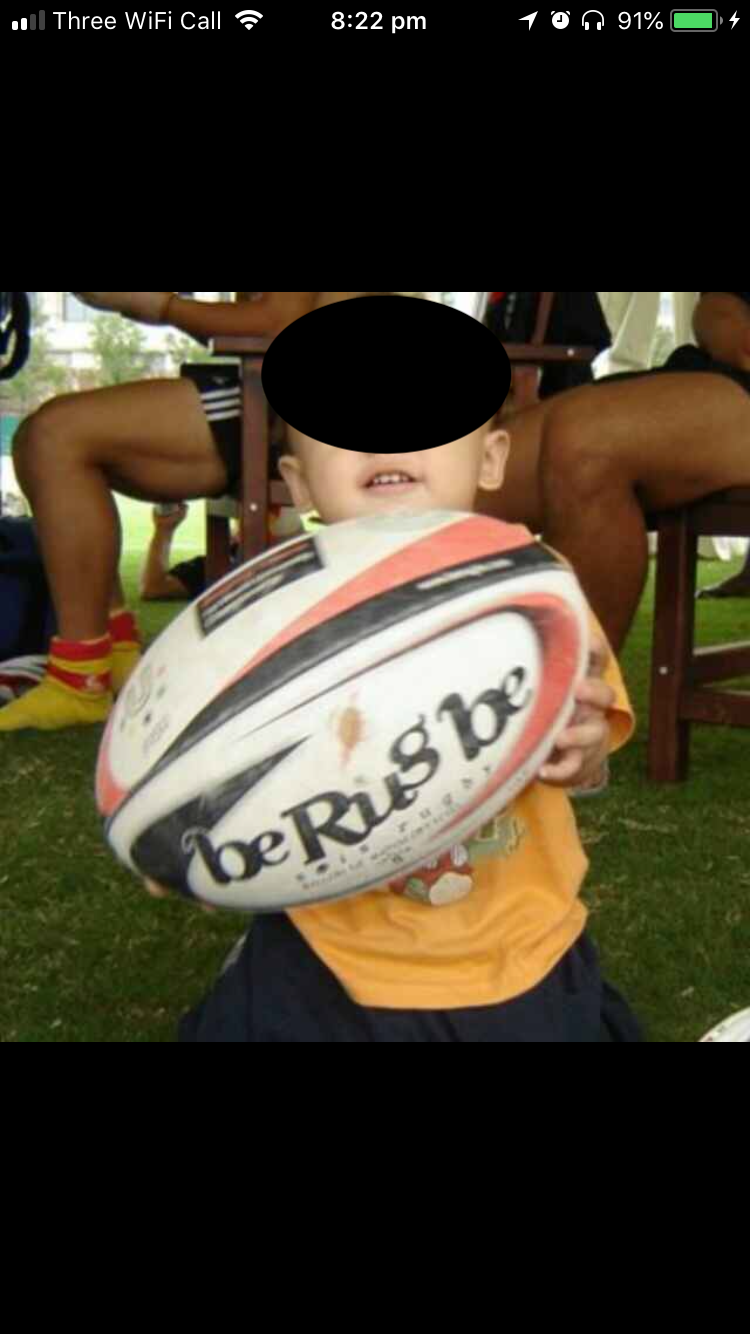
\includegraphics[scale =.2]{images/bjmWeChatProfile1.png}
                    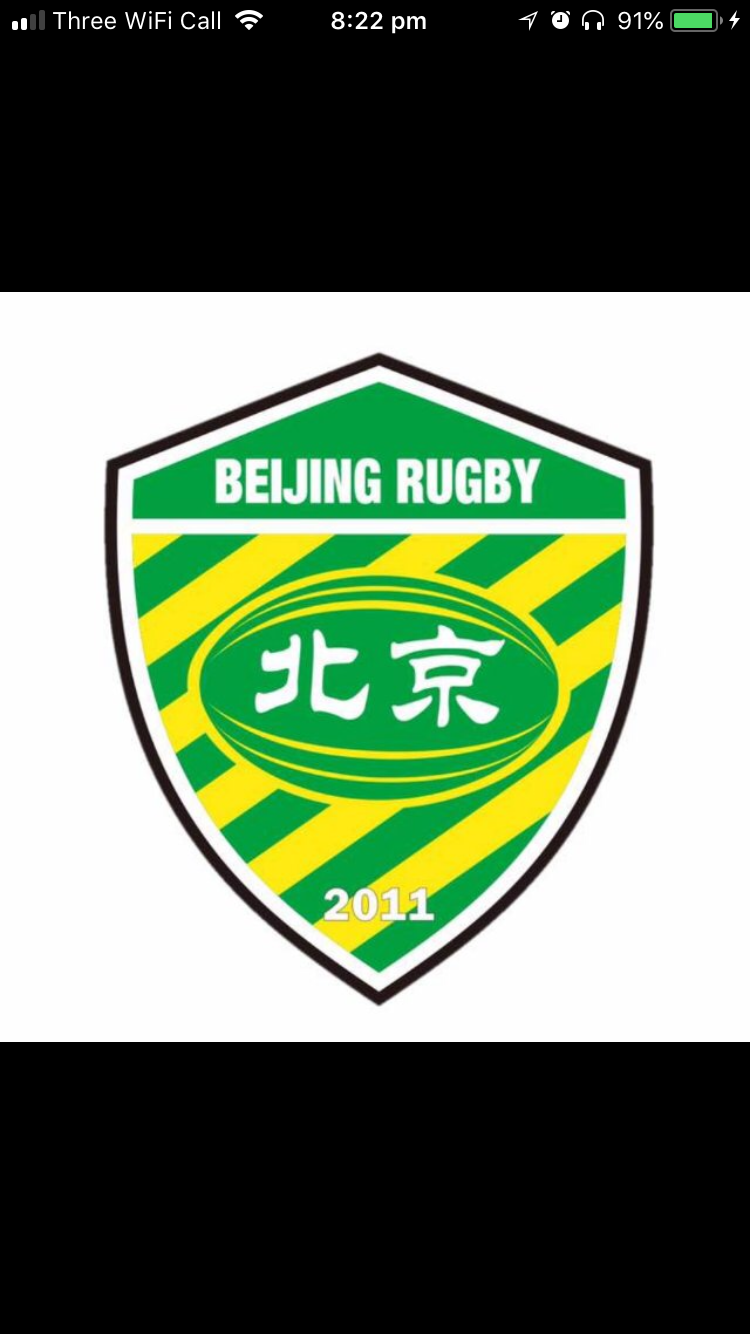
\includegraphics[scale =.2]{images/bjmWeChatProfile2.png}
                    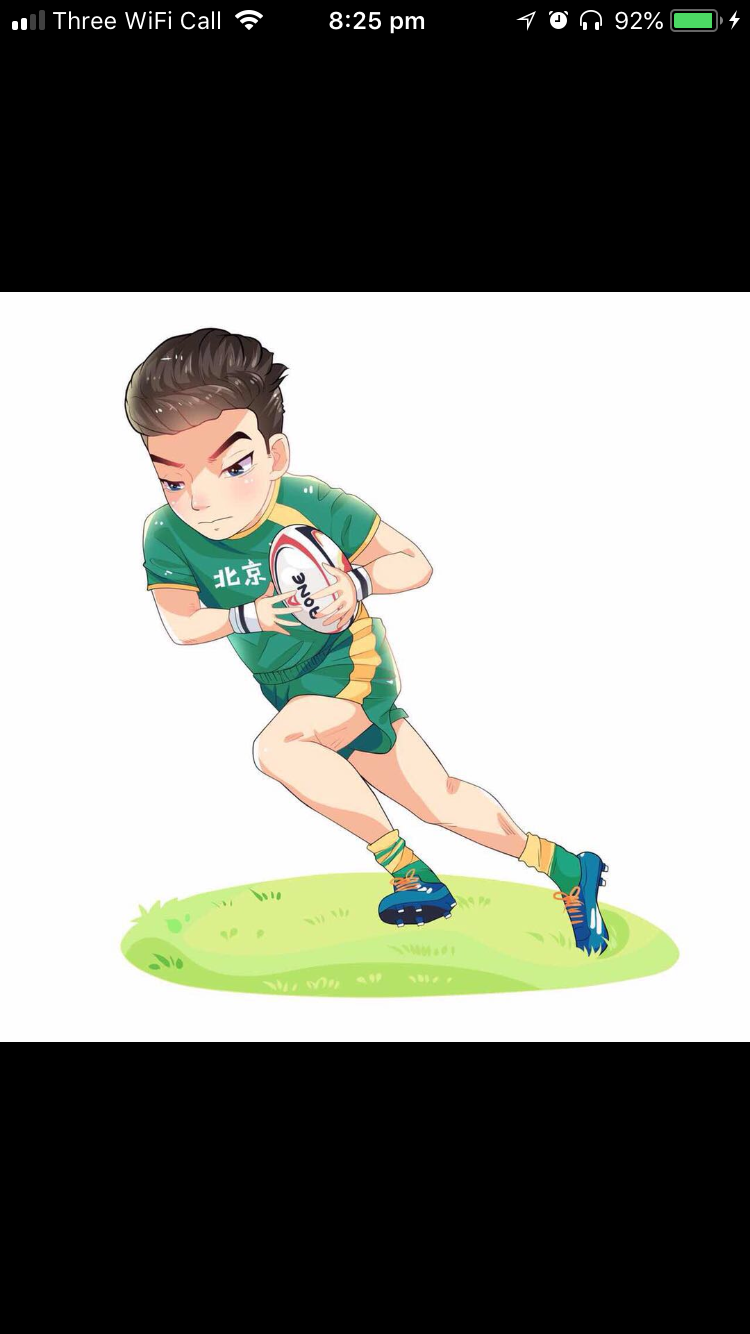
\includegraphics[scale =.2]{images/bjmWeChatProfile3.png}
                    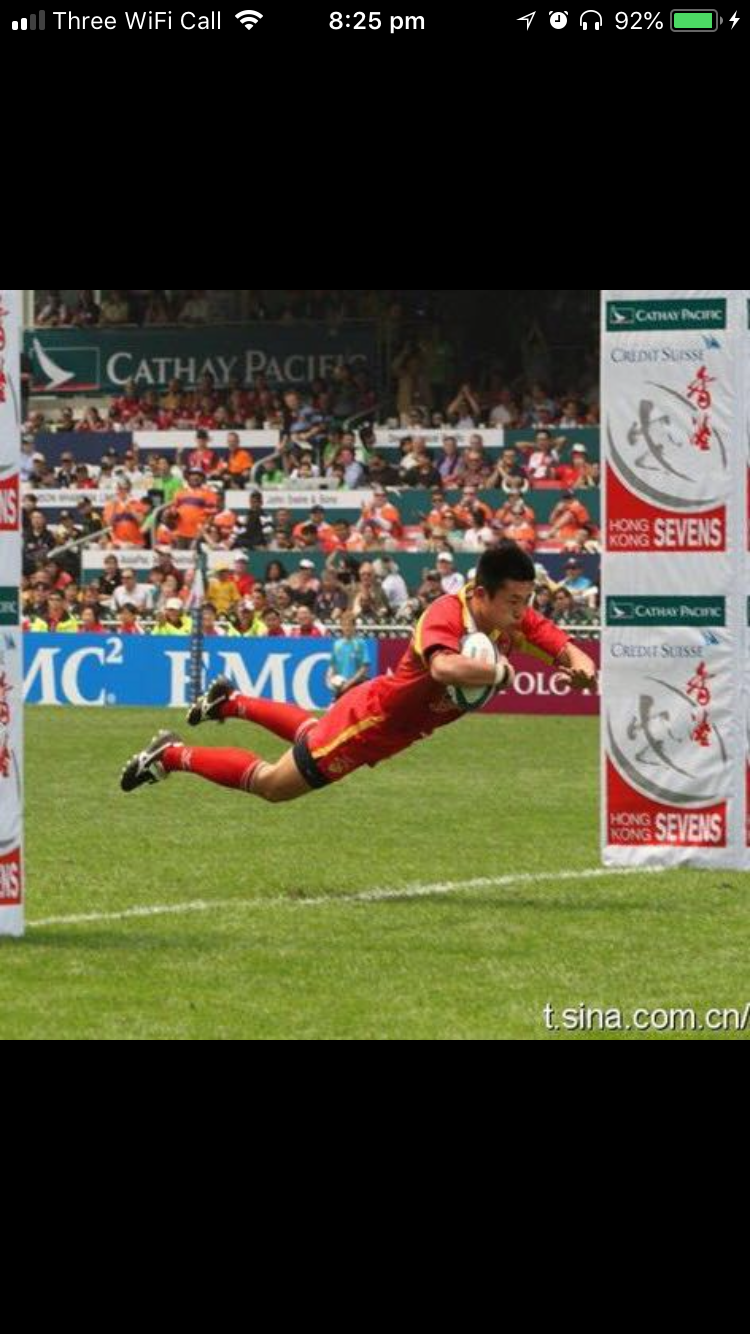
\includegraphics[scale =.2]{images/bjmWeChatProfile4.png}
                    \caption{Screen shots taken from the social media profiles of a selection of athletes}
                  \end{center}
                    \label{fig:bjmWeChatProfile}
                \end{figure}

                %\myparagraph{Signalling on social media}

Taken together, this evidence suggests that, despite strategic and particularistic concerns of athletes to their respective relational networks beyond the rugby team at the Institute, the rugby team at the Institute was a salient and meaningful construct to which



\subsubsection{The team as a relational construct}
While the team was a salient construct for athletes, it was clear that the team did not function to organise physical movement and social communication in the ways that I had come to expect in teams that I had occupied previously.  Over time, I discovered that the team was imbued with a relational logic: it was understood to be hierarchical, distributed throughout people and spaces beyond the 26 athletes, and it was understood to require an ethic of personal-cultivation in order to sustain and enhance membership.  Understanding of the relational logic of social coordination at the institute helped me understand that at times.

  \myparagraph{Team as family, teammates as brothers}
The concept of ``family'' was central to the rugby program's public discourses surrounding social norms of group membership.
From vice-principal Jenny, to the head coaches, and the athletes themselves, family was the metaphor most commonly used to convey the requirements of each athlete to their team.  More so than the egalitarian construct of team, the metaphor of family contained room for expressing both the solidarity and emotional support of shared membership, as well as a justification for the hierarchical structure of the group.  Thus, while the notion of the team was salient in athlete experience, it also appeared that the team may have been construed in relational terms more closely resembling an hierarchical family.  The prominence of conventions associated with family were identifiable in the naming conventions of the team.  As a general rule, when directly addressing elder athletes, an athlete would add the suffix ``\textit{ge}'' (哥) to the elder athlete's first or last name, to indicate that the elder athlete was relationally equivalent to an elder brother.  When addressing Han Xiaolong, the most senior athlete in the group, for example, athletes would commonly use \textit{Long Ge} (龙哥).  When referring to the coach, on the other hand, athletes would use either the formal and respectful ``Teacher'' (\textit{Laoshi} 老师), ``Coach'' (\textit{jiaolian} 教练), or the more colloquial suffix abbreviation of \textit{dao}(导).  The naming conventions for the coach conventions for the coach derived from a Confucian tradition of master-apprentice relationships---originally structured on familial relationship conventions \citep{Spence1999}.
When referring to a teammate in the third person, athletes would often refer to them as either their senior apprentice \textit{Shige} (师哥) or junior apprentice \textit{Shidi}(师弟), depending on whether the teammate was older or younger.  The network of relationships of the rugby team were thus modelled using hierarchical familial and Confucian master-apprentice relational conventions.

Senior athlete Wang Wei offered his perspective on the family-like structure of the rugby program at the Institut

    \begin{quote}
      Its not as if there was not a lot of new stuff, because I guess at the time I was playing basketball---basketball is also a team sport.  But the only little bit that rugby made me experience was respect for elders, newcomers must respect senior team members, senior members must take care of junior team members, this is something that I didn't experience in basketball.  At the time also I didn't understand that much, I guess China has always had respect for elders, but it didn't come up for me in basketball, and so then when I came to rugby my experience of it was very deep.
    \end{quote}

    \begin{quote}
       那倒没有很多,因为我当时打篮球嘛。篮球也是集体项目但是唯一一点和橄榄球比让我体会到就是长幼尊卑,新人得尊重老队员,老队员得关照小队员,这是我在篮球上面没体会过的。当时也没了解这么多,中国文化一直有尊老爱幼嘛,在篮球队没体现过,然后到橄榄球队还是体验特深的。
    \end{quote}
Wang Wei first arrived at the Institute in 2011, during a time when the range in ages of athletes at the program would have been quite extreme, with the youngest athletes being around 16 years old, and the oldest athletes being in their mid 30s (the age range of athletes during my research was 15-28 years).
The hierarchical and relational conventions associated with family functioned as a resource that enabled Wang Wei to navigate the social terrain of group membership in which within-group variation in seniority and experience were high.

Family was also commonly deployed by coaches and the Institute leadership to convey ethics of team commitment.  In an official team meeting approximately two months into my first stint of fieldwork, vice principal Jenny provided the most elegant and articulate example of discursively framing the group as a family.
      \begin{quote}
        ...I very much welcome everyone to join the Institute's rugby team. I also hope that in study, living, and training, everyone will treat each other like their own siblings, with mutual tolerance and understanding.  I hope you are able to create a very good team atmosphere, and it is by no means easy, because everyone comes from all corners of the world. Everyone is an independent individual, more or less autonomous, prone to be relatively selfish, and may also have poor self-management skills.  But this all changes when everyone comes to this big family, because rugby is a team sport. In a team sport, everyone in the team needs to be twisted together into one single rope in order for that rope to send out a force. I don't wish to see cliques of twos and threes; or see you take the field with seven hearts, or with five hearts---rugby doesn't work like that. I wish that [when you take the field] everyone shares only one heart. Only in this way will our team be able to achieve good results.
      \end{quote}
      \begin{quote}
        ...非常欢迎大家加入橄榄球的队伍,也希望在以后学习生活训练过程中希望大家像亲兄弟姐妹一样,互相宽容互相帮助互相体谅,能够形容一个非常好的气氛,因为大家来自五湖四海,非常不容易。每个人都是独立的个体,多多少少都比较自主、比较自私、可能自我管理能力较差。来到这个大家庭之后,因为橄榄球是个团体的项目、团队的项目,需要大家队伍要拧成一股绳,发出一股力。我不希望大家三个一群两个一伙,上场之后七条心、五条心、不是这样。我只希望大家一条心。只有这样我们队伍才能打出好成绩。
      \end{quote}

Taken together, these excerpts suggest that the concept of family offered dual affordances for processes of group membership.  On the one hand, the family represents a group in which every member contributes to and receives collective strength and support, by virtue of the solidarity achieved through group membership.  On the other hand, the family, and indeed, the team, entails hierarchy.  In the formal setting of the team meeting, Jenny emphasised the former dimension of the family.  But it was clear from behaviours in less formal settings that the family also afforded attention to fostering hierarchy, whereby some individuals enjoyed privileged access to shared resources by virtue of their seniority.  The concept of team and its associated egalitarian ethics were, by contrast, insufficient as affordances for explicitly representing and navigating the dominant mode of hierarchical relationism at the Institute, and in a Chinese relational mode of social cognition more generally.


\subsubsection{The entire system must be aligned \label{sect:systemAligned}}
I encountered a number of instances in which it appeared that athletes perceived social coordination to extend well beyond the interplay of immediate social categories of self and the group.  One example occurred the first morning I arrived back for the second major stint of ethnography in the summer of 2016.


\subsubsection{The ``I'' in team \label{sect:IinTeam}}
In addition to emphases on hierarchical relationism in group membership, it became apparent that athletes also emphasised personal cultivation as a means to demonstrate team commitment.  As explained in Chapter ~\ref{chap:researchSetting}, a relational mode of group membership will not always predict deference to others.  In particular, a Chinese relational mode of social cognition predicts that personal cultivation is an equally important component to group membership.

I noticed various instances in which athletes opted to promote the self in social settings as an ethic of group membership.  My realisation of this pattern started during interviews, when I would ask about each athletes' journey to rugby.  Although athletes would recognise in passing the agency of their coach or close relation who facilitated their journey to the Institute, when I asked whose final decision it was to play rugby, almost all athletes would emphasise that coming to the Institute was ultimately their own personal decision.  Often this personal agency was made in counter-distinction to their parent's will.

Senior athlete, Ma Haitao, after explaining how he had been introduced to rugby via one of his family friends (who had attended CAU), explained how he came to the decision to play rugby:
     \begin{quote}
       My Father didn't know this sport.  Because in China very rarely will people know what [rugby] is, so my Parents didn't know. From a young age I've been away from home playing sport, and so generally I decide these things myself...I made the decision myself.  At the time I arrived wheeling a suitcase and had a bag on my back.  I came at the time with a classmate...
     \end{quote}
     \begin{quote}
       我爸不知道这个项目。因为中国很少知道有这个,他们不知道。我从小就在外面练体育,所以我一般是自己决定这些东西\textellipsis自己决定的。当时自己背个包投的箱子来。当时和一个同学,他是农大的。
     \end{quote}

  While not wanting to discount the possibility that Ma's was completely independent in his decisions, it is obvious that Ma's account involves a deliberate emphasis on personal agency, even though at the time to which he was referring he would have still been a legal minor and completely dependent in financial and other senses to his legal guardians (parents and coaches).

  Meng Cheng, a junior aspiring athlete from Beijing's outer suburbs was even more proud that the decision to play rugby was his own:
       \begin{quote}
         My parents at the time thought [rugby] was quite dangerous, and they didn't let me play.  But they weren't as stubborn as I was.  It's the case with everything, I decide...If I to do something I have to make the decision myself, and then no one can change my decision\textellipsis
       \end{quote}
       \begin{quote}
         父母当时觉得很危险,不让我练。但是拗不过我,他什么事都。我自己决定了\textellipsis
         就是说我拿什么我一定拿的主意,任何人改变不了\textellipsis
       \end{quote}

  Pan Qiyu, a senior athlete and CAU graduate from Dandong in Liaoning province, also had a similar story about self-determination when I asked him about his decision to play rugby:
     \begin{quote}
       I decided myself\textellipsis How I came to the decision was actually quite interesting.  At the time when we first came in it was really difficult.  At the time forty or more of us were selected, but many people wouldn't let us train, including our head teacher at high school.  A lot of class teachers said to me that there was no hope for rugby, rugby in China has no development [potential], and there are barely any universities that you can attend [through their rugby programs].  And so then they wouldn't let us (the students who selected rugby) train, only us! After that I said to my Mum and Dad that I really liked this sport, and then my parents also extremely supported me with this.  When I got in to CAU (through their rugby program) my parents were extremely supportive.
    \end{quote}

     \begin{quote}
       我自己做的决定\textellipsis决定特别有意思。当时我们进来的时候特别艰难,当时我们选了四十多个人,好多人不让我们练,包括我们的班主任,好多授课老师跟我说没什么希望,橄榄球在中国没有什么发展, 也没有几所大学能上。然后不让我们练,就——我们! 后来我就跟我爸妈说我特别喜欢这个项目,然后我爸妈也非常支持我,我靠农大的时候他们非常支持我。
     \end{quote}

The pattern of athletes emphasising their own determination in the decision to play rugby was striking, particularly when combined with the fact that almost all athletes also mentioned---more incidentally and as matter-of-fact---that their coaches played some sort of role in facilitating the opportunity to play rugby.  In other words, it was unlikely that these individuals were the sole determiners of the decision.  It was clear that there was some social utility to emphasising self-determination, as if it was an important virtue of group membership.

%P(KIDS):
The virtue of self-determination and self-reliance was powerfully illustrated to me outside the context of the Institute, when I agreed to help out CAU coach (and China's most famous rugby player Johnny Zhang) by agreeing to take a rugby session with a group of young school children (aged between six and eight years).

The training session was designed to be explicitly educational, and so I felt that I should attempt to tie some of the elements of team work in rugby to virtues of friendship and cooperation.  Towards the end of the session, when trying to emphasise the importance of teamwork in a team relay drill, I asked the children: ``Who do you rely on most in this life?'' (你在生活中最依赖谁?).  I was hoping that this question would naturally prompt the answer that they had to rely most on their family and friends for support---what I thought was a relatively obvious response in either a Confucian or Anglo-Protestant system of ethics!).  To my surprise, a chorus of two or three more outspoken children responded, instead: ``Myself!'' (自己!) We rely most in life on the self, these kids insisted. Self-reliance was not the reply I was looking for, but it did say something about the emphasis on self-reliance as an important virtue of group membership.  Indeed, consultation of Chinese indigenous psychology reveals that personal cultivation is a central virtue in a Confucian system of ethics, and is a central resource necessary to foster viable social relationships \citep{Liu2014}.

The active cultivation of the self was a recurrent theme in interviews with athletes when asking about their role in the team and how they ought best contribute to the team.  As unruly undergrad Hou Siqi explained when I asked him if he considered his teammates as an important part of his motivations for adherence to rugby:
   \begin{quote}
       I think about them (teammates) little bit, but I think after all the main thing is to make sure you do a good job your self.  When you're looking after your self that can be a foundation on which to consider others.
   \end{quote}
   \begin{quote}
         有一点,但是我觉得我毕竟是主要还是想把自己做好,做好自己的基础上为再考虑大家.
   \end{quote}

When I asked another unruly undergrad, Fang Chao, about his perceived role in the team, and what he ought to focus on, he responded that he ``hadn't thought that much about it, I just want to make sure I play well myself, ensure that I personally train hard'' (我没想那么多,就想自己把球打好,自己好好练).
In all of these instances, personal cultivation appears to function as an ethic of group membership.
In contrast to a

\section{Discussion}


  Perhaps one of the most powerful distillations of the team came in the form The prominence of personal cultivation as a social virtue was assertion and promotion within the context of the team was performed at a team dinner held on a Sunday night (when everyone had returned from leave) a few weeks after Wang took the reigns as head coach.

Han's speech appeared to me to be a deeply self-promotional act (at the expense of an egalitarian ethic of equal access to the resources of team membership). But this interpretation is generated from my inherently categorical intuitions concerning social processes such as group membership.

Considered from the perspective of a dominant relational mode of social cognition, Han's speech cab be interpreted as being deeply prosocial, as it expressed expressed that he was upholding his part in the system of hierarchically structured relationships that made up the Beijing men's rugby team.  In this way, Han's dream was the group's dream, and Han's prosociality needed not to be mediated through reference to the category of team or egalitarian membership to that category \citep{Liu2009}.

This is not to say that identification with social categories such as the team were not meaningful or functional in processes of group membership. It was clear that they were.  Later in the evening, as the speeches progressed around the table, I did hear some of the more junior senior players make reference to team ideals.  CAU graduate Pan Qiyu suggested in his speech that ``we all need to put ourselves after the team; this is a team sport'' (我们都有把自己放在团队之下); and old head Wang Wei: ``this is a team sport; team first, self second'' (这是个团队项目。团队第一,自己第二).  Importantly, however, these assertions were not egalitarian in their essence, and instead suggested an individual subservience to the team, rather than an egalitarian, shared ownership of the team by each of its members (a more common notion expressed in Western team sport contexts that I have been a part of previously).

Indeed, when Pan and Wang were referring to the team, it could be assumed that what they had in mind was a relational network of individuals structured in a fashion that mirrored the seating arrangement. On one level, the team was united together as equals: all of its members sat at a round table in which everyone had a seat. But on another level, this circle was imbued with a hierarchical structure through which relations of power that flowed from the coach at one end to the most tenuous and junior athlete sat nervously awaiting orders at the other end.  Both relational and categorical modes of group membership were functional resources in processes of social coordination












            \end{CJK}
